\documentclass[11pt,a4paper]{article}

\usepackage[utf8]{inputenc}
\usepackage[T1]{fontenc}
\usepackage{lmodern}
\usepackage[margin=2.5cm]{geometry}
\usepackage{amsmath,amssymb}
\usepackage{booktabs,tabularx,array}
\usepackage{xcolor}
\usepackage{tikz}
\usetikzlibrary{positioning,arrows.meta,fit,backgrounds,shapes.geometric,calc}
\usepackage{listings}
\usepackage{enumitem}
\usepackage{caption}
\usepackage{float}
\usepackage{fancyhdr}
\usepackage[hidelinks]{hyperref}

% --- Nombres en español (sin babel) ---------------------------------------
\renewcommand{\contentsname}{Índice}
\renewcommand{\tablename}{Tabla}
\renewcommand{\figurename}{Figura}
\renewcommand{\refname}{Referencias}
\renewcommand{\lstlistingname}{Código}

\definecolor{azul}{HTML}{1F4E79}
\definecolor{verde}{HTML}{2E7D32}
\definecolor{rojo}{HTML}{C62828}
\definecolor{naranja}{HTML}{EF6C00}
\definecolor{gris}{HTML}{F4F6F8}

\lstset{
  language=Python, basicstyle=\ttfamily\footnotesize, keywordstyle=\color{azul}\bfseries,
  commentstyle=\color{gray}\itshape, stringstyle=\color{verde}, backgroundcolor=\color{gris},
  frame=single, rulecolor=\color{gray!40}, breaklines=true, numbers=left,
  numberstyle=\tiny\color{gray}, showstringspaces=false, inputencoding=utf8, extendedchars=true,
  literate={á}{{\'a}}1 {é}{{\'e}}1 {í}{{\'i}}1 {ó}{{\'o}}1 {ú}{{\'u}}1 {ñ}{{\~n}}1
           {Á}{{\'A}}1 {É}{{\'E}}1 {Í}{{\'I}}1 {Ó}{{\'O}}1 {Ú}{{\'U}}1
}

\pagestyle{fancy}
\fancyhf{}
\lhead{\small Agente DevOps de revisión de Pull Requests}
\rhead{\small Tecnology Trend}
\cfoot{\thepage}

\newcommand{\Pdef}{P_{\text{def}}}

\begin{document}
\sloppy

% ============================== PORTADA ===================================
\begin{titlepage}
\centering
{\large FUNDACIÓN UNIVERSITARIA LOS LIBERTADORES\par}
{\large Facultad de Ingeniería y Ciencias Básicas\par}
{\large Ingeniería de Sistemas\par}
\vspace{3cm}
{\Huge\bfseries Agente Inteligente de Revisión de Código y Gestión de Pull Requests\par}
\vspace{0.6cm}
{\Large Proyecto 4 --- DevOps\par}
\vspace{0.4cm}
{\large Taller de Ingeniería de Agentes Inteligentes\par}
\vspace{0.3cm}
{\large\itshape Entrega 1: Contexto del problema, entorno y modelo PEAS\par}
\vspace{3cm}
{\large\textbf{Presentado por:}\\ Simon Hurtado\par}
\vspace{0.8cm}
{\large\textbf{Docente:}\\ Profesor Gonzalo\par}
\vspace{0.8cm}
{\large\textbf{Asignatura:}\\ Tecnology Trend\par}
\vfill
{\large Bogotá D.C., noviembre de 2026\par}
\end{titlepage}

\tableofcontents
\newpage

% ============================== 1 =========================================
\section{Introducción y contexto del problema}

En los equipos de desarrollo ágil la revisión manual de código suele convertirse en un cuello de
botella: los Pull Requests (PR) esperan horas o días a que un revisor esté disponible, lo que retrasa
los despliegues. Aprobar cambios sin validación rigurosa, en cambio, introduce vulnerabilidades y
errores en producción.

El objetivo de este proyecto es construir un \textbf{agente inteligente integrado en el flujo de
integración continua (CI/CD)} que evalúe cada PR y decida de forma autónoma entre cuatro acciones:
\textit{aprobar y fusionar}, \textit{solicitar correcciones}, \textit{asignar a un arquitecto senior}
o \textit{bloquear el despliegue}. La decisión se toma maximizando una función de utilidad que
resuelve el dilema central del proyecto:

\begin{center}
\fbox{\parbox{0.85\textwidth}{\centering\textbf{Dilema de utilidad:} acelerar la velocidad de entrega
continua de software frente al riesgo de introducir defectos críticos en producción.}}
\end{center}

El prototipo se implementó en Python siguiendo la plantilla del taller y se conectó a GitHub Actions,
de modo que el agente puede operar sobre repositorios reales: lee los artefactos del pipeline, calcula
la utilidad de cada acción, comenta el PR y deja el \textit{check} en verde o en rojo.

% ============================== 2 =========================================
\section{Formalización del entorno y modelo PEAS}

\subsection{Modelo PEAS}

\begin{table}[H]
\centering
\caption{Especificación PEAS del Agente DevOps.}
\label{tab:peas}
\begin{tabularx}{\textwidth}{@{}l X@{}}
\toprule
\textbf{Componente} & \textbf{Aplicación al agente} \\
\midrule
\textbf{Performance} & Reducción de fallos tras el despliegue (defectos escapados = 0), disminución del
tiempo de ciclo de aprobación y cumplimiento de estándares de calidad (cobertura $\geq 70\,\%$, cero
vulnerabilidades críticas, pruebas en verde). \\
\addlinespace
\textbf{Environment} & Repositorios Git (GitHub), pipelines de CI/CD (GitHub Actions), entornos de
pruebas automatizadas (pytest), herramientas de análisis estático (Bandit) y el equipo de
desarrolladores y arquitectos. \\
\addlinespace
\textbf{Actuators} & Aprobar y fusionar (\textit{merge}) el código, publicar comentarios con
sugerencias técnicas, etiquetar el PR, poner el \textit{check} en rojo para bloquear el despliegue y
asignar revisores humanos. \\
\addlinespace
\textbf{Sensors} & Líneas modificadas y archivos tocados (\texttt{git diff --numstat}), reporte de
pruebas unitarias (JUnit XML), cobertura de código (\texttt{coverage.json}), alertas de análisis
estático de seguridad (Bandit) y rama de destino. \\
\bottomrule
\end{tabularx}
\end{table}

Cada sensor se transforma en un atributo normalizado del objeto \texttt{SensoresPR}, lo que separa
claramente \emph{lo que el agente percibe} (sensores) de \emph{lo que el agente hace} (actuadores).

\subsection{Propiedades del entorno}

\begin{table}[H]
\centering
\caption{Clasificación del entorno de trabajo.}
\label{tab:entorno}
\begin{tabularx}{\textwidth}{@{}l l X@{}}
\toprule
\textbf{Propiedad} & \textbf{Valor} & \textbf{Justificación} \\
\midrule
Observabilidad & Parcial & El diff, las pruebas y el SAST no revelan todos los defectos: un PR con
pruebas en verde puede contener errores lógicos no cubiertos. El agente debe \emph{estimar}
$\Pdef$. \\
Determinismo & Estocástico & La misma acción puede tener resultados distintos: un merge de bajo riesgo
puede, con cierta probabilidad, provocar un incidente en producción. \\
Dinamismo & Dinámico & Mientras el agente evalúa, llegan nuevos commits al PR, la rama
\texttt{main} cambia y otros PRs compiten por el pipeline. \\
Episodios & Secuencial & Fusionar código defectuoso afecta a los PRs futuros (deuda técnica,
conflictos, regresiones). \\
Variables & Discreto / continuo & Las acciones son discretas (4); los sensores son continuos
(cobertura, proporción de pruebas). \\
Agentes & Multiagente & Interactúa con desarrolladores, arquitectos y otros bots de CI (Dependabot,
linters). \\
\bottomrule
\end{tabularx}
\end{table}

\subsection{Diagrama de contexto}

\begin{figure}[H]
\centering
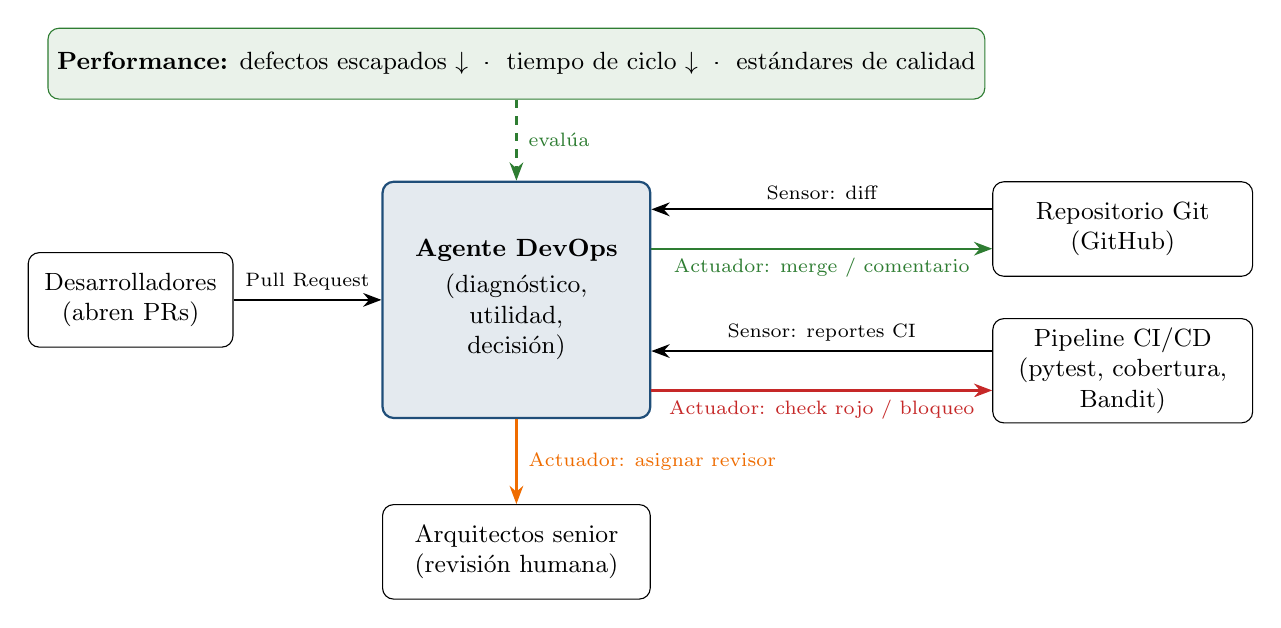
\begin{tikzpicture}[>=Stealth, font=\small,
  caja/.style={draw, rounded corners, align=center, fill=white, minimum height=1.2cm},
  flecha/.style={->, thick}, et/.style={font=\scriptsize, fill=white, inner sep=1pt}]
\node[caja, fill=azul!12, draw=azul, thick, minimum width=3.4cm, minimum height=3cm] (ag) at (0,0)
  {\textbf{Agente DevOps}\\[2pt](diagnóstico,\\utilidad,\\decisión)};
\node[caja, minimum width=2.6cm] (dev) at (-4.9,0) {Desarrolladores\\(abren PRs)};
\node[caja, minimum width=3.3cm] (repo) at (7.7,0.9) {Repositorio Git\\(GitHub)};
\node[caja, minimum width=3.3cm] (ci) at (7.7,-0.9) {Pipeline CI/CD\\(pytest, cobertura,\\Bandit)};
\node[caja, minimum width=3.4cm] (arq) at (0,-3.2) {Arquitectos senior\\(revisión humana)};
\node[caja, fill=verde!10, draw=verde, minimum width=9cm, minimum height=0.9cm] (perf) at (0,3)
  {\textbf{Performance:} defectos escapados $\downarrow$ \;·\; tiempo de ciclo $\downarrow$ \;·\; estándares de calidad};
% desarrolladores
\draw[flecha] (dev.east) -- node[et, above=2pt]{Pull Request} (ag.west);
% repositorio: sensor (arriba) y actuador (abajo)
\draw[flecha] (repo.west |- 0,1.15) -- node[et, above=2pt]{Sensor: diff} (ag.east |- 0,1.15);
\draw[flecha, verde] (ag.east |- 0,0.65) -- node[et, below=2pt, text=verde]{Actuador: merge / comentario} (repo.west |- 0,0.65);
% pipeline: sensor (arriba) y actuador (abajo)
\draw[flecha] (ci.west |- 0,-0.65) -- node[et, above=2pt]{Sensor: reportes CI} (ag.east |- 0,-0.65);
\draw[flecha, rojo] (ag.east |- 0,-1.15) -- node[et, below=2pt, text=rojo]{Actuador: check rojo / bloqueo} (ci.west |- 0,-1.15);
% arquitectos y performance
\draw[flecha, naranja] (ag.south) -- node[et, right=3pt, text=naranja]{Actuador: asignar revisor} (arq.north);
\draw[flecha, dashed, verde] (perf.south) -- node[et, right=3pt, text=verde]{evalúa} (ag.north);
\end{tikzpicture}
\caption{Interacción del Agente DevOps con su entorno.}
\label{fig:contexto}
\end{figure}

\begin{thebibliography}{9}
\bibitem{russell} S. Russell y P. Norvig, \textit{Artificial Intelligence: A Modern Approach}, 4.ª ed. Pearson, 2021.
\bibitem{taller} \textit{Taller de Ingeniería de Agentes Inteligentes: de los fundamentos a los sistemas multiagente}. Material de clase, noviembre de 2026.
\end{thebibliography}

\end{document}
